%%%%%%%%%%%%%%%%%%%%%%%%%%%%%%%%%%%%%%%%%%%%%%%%%%%%%%%%%%%%%%%%%%%%%%%%
% This is the main file of the Msc thesis template.
%%%%%%%%%%%%%%%%%%%%%%%%%%%%%%%%%%%%%%%%%%%%%%%%%%%%%%%%%%%%%%%%%%%%%%%%
%
% Author:   René Widmer
%           Institute for Surgical Technology and Biomechanics ISTB
%           University of Bern
%           rene.widmer@istb.unibe.ch
%
% Date:     10/28/2009
%
%%%%%%%%%%%%%%%%%%%%%%%%%%%%%%%%%%%%%%%%%%%%%%%%%%%%%%%%%%%%%%%%%%%%%%%%

\pdfminorversion=6
\documentclass[a4paper,10pt,openright]{unibe-msc}
% Some regulary used packages
\usepackage{etex}
\usepackage[T1]{fontenc}
\usepackage{textcomp}
\usepackage{bm}
\usepackage[utf8]{inputenc}
\usepackage[pdftex,final]{graphicx}
\usepackage{amssymb}
\usepackage{amsmath}                    
\usepackage{amsfonts}
\usepackage{mathtools}
\usepackage{ulem}
\usepackage[english]{babel}
\usepackage{url}
\usepackage{color}
%\usepackage{unibe-msc}
\usepackage[caption=off]{subfig}
\usepackage{hyperref}


% Default graphics path
%\graphicspath{{Images/}{Logos/}}

% Document metadata
\unibelogo{ub_16pt_192}  % Don't change this
\htilogo{TI_eps} % Don't change this
\faculty{Faculty of Medicine} % Don't change this
\discipline{Biomedical Engineering} % Don't change this
\subtitle{Master of Science Thesis} % Don't change this
\title{Probabilistic Stimulation Maps for Deep Brain Stimulation}
\author{Quentin Savary}
\origin{Switzerland}
\date{\today}
\supervisor{Dr. T. A. Khoa Nguyen and Prof. Claudio Pollo}
\affiliation{ARTORG Center for Biomedical Engineering Research, Universit\"{a}t Bern Department of Neurosurgery, Inselspital Bern}

\examiner{Prof... }
\place{Bern}
\frontsignature{\theplace, October 2009}
\date{October 31\textsuperscript{th} 2009}

%%%%%%%%%%%%%%%%%%%%%%%%%%%%%%%%%%%%%%%%%%%%%%%%%%%%%%%%%%%%%%%%%%%%%
% Hyperref setup
%%%%%%%%%%%%%%%%%%%%%%%%%%%%%%%%%%%%%%%%%%%%%%%%%%%%%%%%%%%%%%%%%%%%%
% Appearance of hyper links
\definecolor{lc}{rgb}{0,0,0}
\hypersetup{colorlinks=true, breaklinks=true, linkcolor=lc, 
                  menucolor=lc, urlcolor=lc, anchorcolor=lc,
                  citecolor=lc, filecolor=lc,
                  pdftitle=\thetitle,
                  pdfauthor=\theauthor,
                  pdfsubject=Master Thesis,
                  pdfkeywords={Keyword 1, Keyword 2, Keyword 3},
                  pdfpagelayout=SinglePage}
                  
% Bibliography style file
\bibliographystyle{ieee}

\begin{document}

%%%%%%%%%%%%%%%%%%%%%%%%%%%%%%%%%%%%%%%%%%%%%%%%%%%%%%%%%%%%%%%%%%%%%
% Titlepage, abstract table of contents etc.
%%%%%%%%%%%%%%%%%%%%%%%%%%%%%%%%%%%%%%%%%%%%%%%%%%%%%%%%%%%%%%%%%%%%%
\frontmatter
\maketitle
%%%%%%%%%%%%%%%%%%%%%%%%%%%%%%%%%%%%%%%%%%%%%%%%%%%%%%%%%%%%%%%%%%%%%%%%
% This is the conclusion chapter file.
%%%%%%%%%%%%%%%%%%%%%%%%%%%%%%%%%%%%%%%%%%%%%%%%%%%%%%%%%%%%%%%%%%%%%%%%
%
% Author:   René Widmer
%           Institute for Surgical Technology and Biomechanics ISTB
%           University of Bern
%           rene.widmer@istb.unibe.ch
%
% Date:     10/28/2009
%
%%%%%%%%%%%%%%%%%%%%%%%%%%%%%%%%%%%%%%%%%%%%%%%%%%%%%%%%%%%%%%%%%%%%%%%%

\begin{abstract}

\noindent\textit{The abstract should provide a concise (300-400 word) summary of the motivation, methodology, main results and conclusions. For example:}

\vskip1em

Osteoporosis is a disease in which the density and quality of bone are reduced. As the bones become more porous and fragile, the risk of fracture is greatly increased. The loss of bone occurs progressively, often there are no symptoms until the first fracture occurs. Nowadays as many women are dying from osteoporosis as from breast cancer. Moreover it has been estimated that yearly costs arising from osteoporotic fractures alone in Europe worth 30 billion Euros.

Percutaneous vertebroplasty is the injection of bone cement into the vertebral body in order to relieve pain and stabilize fractured and/or osteoporotic vertebrae with immediate improvement of the symptoms. Treatment risks and complications include those related to needle placement, infection, bleeding and cement extravazation. The cement can leak into extraosseous tissues, including the epidural or paravertebral venous system eventually ending in pulmonary embolism and death.

The aim of this project was to develop a computational model to simulate the flow of two immiscible fluids through porous trabecular bone in order to predict the three-dimensional spreading patterns developing from the cement injection and minimize the risk of cement extravazation while maximizing the mechanical effect. The computational model estimates region specific porosity and anisotropic permeability from Hounsfield unit values obtained from patient-specific clinical computer tomography data sets. The creeping flow through the porous matrix is governed by a modified version of Darcy's Law, an empirical relation of the pressure gradient to the flow velocity with consideration of the complex rheological properties of bone cement.

To simulate the immiscible two phase fluid flow, i.e. the displacement of a biofluid by a biomaterial, a fluid interface tracking algorithm with mixed boundary representation has been developed. The nonlinear partial differential equation arising from the problem was numerically implemented into the open-source Finite Element framework \textit{libMesh}. The algorithm design allows the incorporation of the developed methods into a larger simulation of vertebral bone augmentation for pre-surgical planning.

First simulation trials showed close agreement with the findings from relevant literature. The computational model demonstrated efficiency and numerical stability. The future model development may incorporate the morphology of the region specific trabecular bone structure improving the models' accuracy or the prediction of the orientation and alignment of fiber-reinforced bone cements in order to increase fracture-resistance. 

\end{abstract}

\endinput

\clearpage
\chapter*{Acknowledgements}
   
\textit{Here you may include acknowledgements.}

\endinput
\clearpage

\vspace*{0cm}
\vfill
\noindent\parbox[b][0.5\textheight]{\textwidth}
{
		\vfill
		\noindent\normalsize\mdseries\itshape
Ich erkläre hiermit, dass ich diese Arbeit selbständig verfasst und keine anderen als die angegebenen Hilfsmittel benutzt habe. Alle Stellen, die wörtlich oder sinngemäss aus Quellen entnommen wurden, habe ich als solche kenntlich gemacht. Mir ist bekannt, dass andernfalls der Senat gemäss dem Gesetz über die Universität zum Entzug des auf Grund dieser Arbeit verliehenen Titels berechtigt ist.\par
		\vspace{2cm}
		\noindent\normalsize\normalfont
		{
			Bern, \thedate\par
		}\par
		\vspace{2cm}
		\noindent\normalsize\normalfont
		{
			\theauthor\par
		}\par
}\par
\cleardoublepage
\tableofcontents

\mainmatter

%%%%%%%%%%%%%%%%%%%%%%%%%%%%%%%%%%%%%%%%%%%%%%%%%%%%%%%%%%%%%%%%%%%%%
% Main text body
%%%%%%%%%%%%%%%%%%%%%%%%%%%%%%%%%%%%%%%%%%%%%%%%%%%%%%%%%%%%%%%%%%%%%
%%%%%%%%%%%%%%%%%%%%%%%%%%%%%%%%%%%%%%%%%%%%%%%%%%%%%%%%%%%%%%%%%%%%%%%%
% This is the introduction chapter file.
%%%%%%%%%%%%%%%%%%%%%%%%%%%%%%%%%%%%%%%%%%%%%%%%%%%%%%%%%%%%%%%%%%%%%%%%
%
% Author:   René Widmer
%           Institute for Surgical Technology and Biomechanics ISTB
%           University of Bern
%           rene.widmer@istb.unibe.ch
%
% Date:     10/28/2009
%
%%%%%%%%%%%%%%%%%%%%%%%%%%%%%%%%%%%%%%%%%%%%%%%%%%%%%%%%%%%%%%%%%%%%%%%%

\chapter{Introduction}

\textit{The introduction provides a thorough review of the background, including relevant literature, the motivation, the aims of the thesis and the hypotheses. Literature references for the thesis should be collected in one common bibliography at the end of the thesis.}

\vskip1em

With the population aging, medicine is recognizing the major impact of osteoporosis on health and function. The chief manifestation of osteoporosis is the pathologic fracture. Osteoporotic patients sustain fractures when minimal force is applied to weakened, discontinuous bone. Traditionally, most attention has been given to osteoporotic fractures of the hip. However, the 700'000 osteoporotic vertebral compression fractures per year in the United States easily outnumber fractures of the hip and ankle combined.

It is estimated that more than 200 million people worldwide are currently affected by osteoporosis, and 100 million are at risk of suffering from related complications. It is a proven fact that solely in Europe about 3.8 million osteoporotic fractures were treated in the year 2000. The prevalence of the disease is expected to rise significantly with the aging population: In the US, the number of annual osteoporosis-attributable fractures is expected to double by the year 2025, and the growth predictions for Switzerland are of comparable magnitude. The total cost of osteoporotic fractures in the US was estimated at 7 - 10 billion dollars in 1995 for a population of 250 million, and expenditures for the treatment of vertebral fractures alone were estimated at 377 million Euros in 2003 in the European Union.

Vertebral compression fractures have previously received limited attention from the spine care community. This oversight may be a result of the perception that vertebral compression fractures are benign, self-limited problems or that treatment options are limited. However, it has become clear that vertebral compression fractures are associated with significant physiologic and functional impairment, even in patients not presenting for medical evaluation at the time of fracture.

Open surgery is fraught with morbidity and implant failure in this frail patient population. Therefore, nonoperative management, including medications and bracing, has been recommended for the vast majority of patients. Unfortunately, large numbers of patients report intractable pain and inability to return to activities. The limitations of nonoperative management have encouraged increasing interest in new, percutaneous methods of fracture stabilization that allow early return to activity and do not require fixation in weak bone.

Percutaneous vertebroplasty was first performed in France in the mid 1980s, and there is extensive experience with the technique in continental Europe. Originally used to treat the painful, aggressive variant of vertebral haemangioma\footnote{A haemangioma describes a benign overgrowth of blood vessels.}, percutaneous vertebroplasty has been applied to painful vertebral lesions caused by metastatic disease and painful osteoporotic fractures.

Osteoporosis is a skeletal disorder which is characterized by loss of bone mass and degradation of trabecular structure, which results in an increased fracture risk. Osteoporotic fractures most frequently occur in structures subjected to large strains, such as the spine or the hip, or bones commonly affected by falls, such as the distal forearm. Thoracic and lumbar vertebral collapses are recognized as the most frequent complication resulting from the loss of bony substance.

\vskip1em
\noindent\textit{etc.}

\begin{figure}[htbp]
	\centering
	\subfloat[Normal]
	{
		\label{fig:subfig:NormalStructure}
		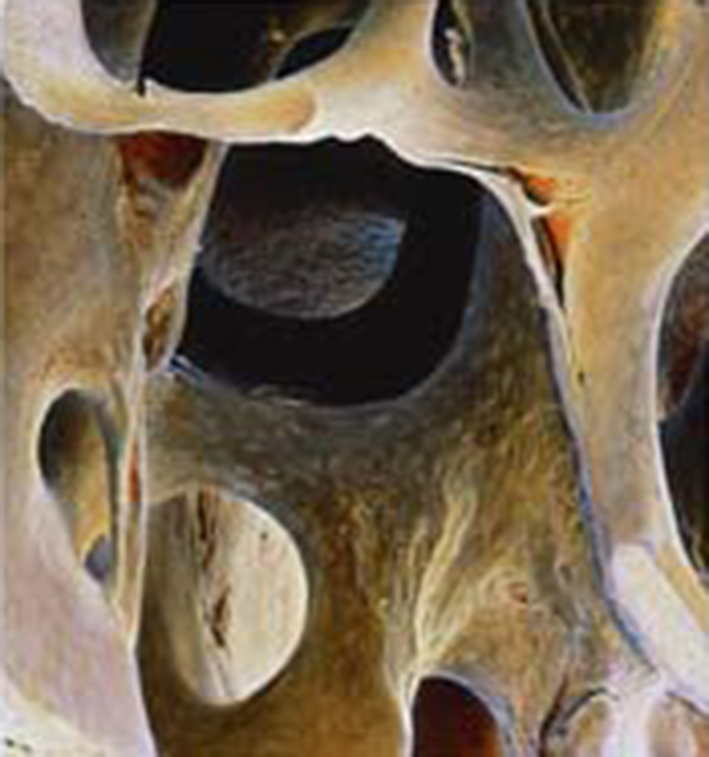
\includegraphics[width=4.5cm]{NormalBoneStructure}
	}
	\hfill
	\subfloat[Osteoporotic]
	{
		\label{fig:subfig:OsteoporoticStructure}
		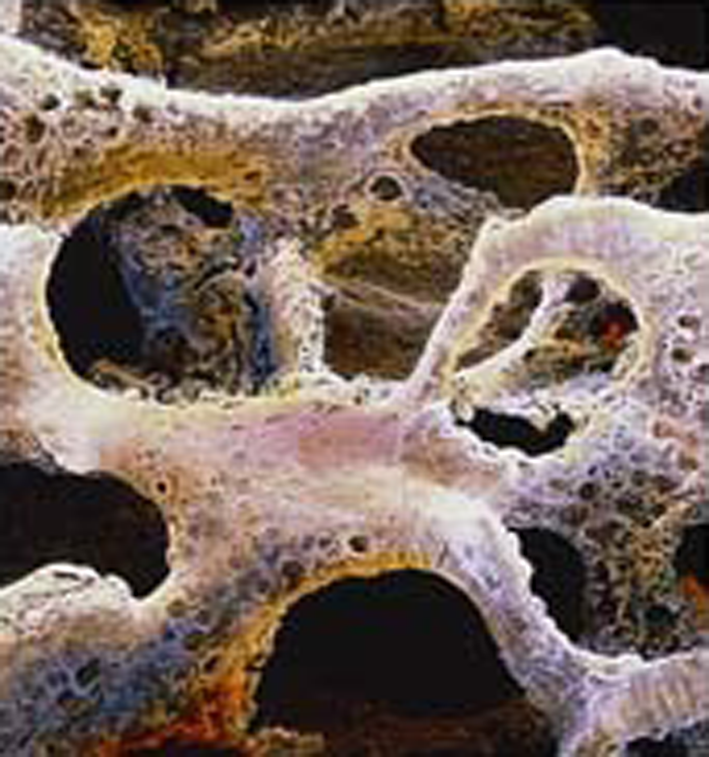
\includegraphics[width=4.5cm]{OsteoporoticBoneStructure}
	}
	\caption[Normal and osteoporotic spongy bone structure]{Normal and osteoporotic spongy microscale bone structure at 25x magnification. Image source: \url{http://facstaff.unca.edu/cnicolay/BIO223-F08/L06-bone.pdf}.\par\vspace{1em}\textit{Please document your image sources.}}
	\label{fig:OsteoporoticStructure}  
\end{figure}


\endinput
%%%%%%%%%%%%%%%%%%%%%%%%%%%%%%%%%%%%%%%%%%%%%%%%%%%%%%%%%%%%%%%%%%%%%%%%
% This is the sample chapter file.
%%%%%%%%%%%%%%%%%%%%%%%%%%%%%%%%%%%%%%%%%%%%%%%%%%%%%%%%%%%%%%%%%%%%%%%%
%
% Author:   René Widmer
%           Institute for Surgical Technology and Biomechanics ISTB
%           University of Bern
%           rene.widmer@istb.unibe.ch
%
% Date:     10/28/2009
%
%%%%%%%%%%%%%%%%%%%%%%%%%%%%%%%%%%%%%%%%%%%%%%%%%%%%%%%%%%%%%%%%%%%%%%%%

\chapter{A Sample Chapter}

\section{A Sample Section with a Table}

\subsection{Porosity Estimation}

Clinical need:
A few weeks after the implantation of the leads, neurologists need to find the optimal contact and parameters in order to obtain the best therapeutic effect. For now, this process is performed with a brute force approach by assessing the clinical outcome of each individual contacts at different stimulation amplitude. The duration of this process takes approximately 4 hours per electrodes or 8 hours per patient. Furthermore, it can be uncomfortable for the patient which is not under medication during the whole process. Another issue is the high cost to pay a neurologist during one day to perform this task. Thus, the clinical need is to reduce this programming time.
In 2019, the team wrote an article, with the data gathered with the past implantation and programming of patients. The generated sweet spot regroups the information of all the data, without distinction of any kind. The age, gender, hemisphere, and other variable could have a significant impact on the sweet spot and may, and 
Some data about essential tremor patient have also been gathered and the fact that the stimulation zone for this disease is larger than for Parkinson raised the question about the number of data needed to obtain a significantly precise stimulation map. 
The map is a representation of the brain containing information about the “probability” of each voxel to be in the sweet spot. It may also contain other information. The sweet spot is defined as the voxels having a probability higher than a given threshold. The VTA are estimation of the volume of tissue activated by stimulation. Those estimation are based on finite-element simulation of electrical field based on the reconstruction of the lead and ?? the 
Vision:
The final goal of this project is to provide a software for neurologist, which takes the pre/post implantation MRI and CT image. This software should give a recommendation about the contact and stimulation parameters. (Not for this project) After the testing and “manual” optimization of the neurologist, the new data could be used to update the stimulation map to increase its accuracy.

\begin{equation}
   v_{m,n,p}\in\left\{0,1\right\}\qquad\forall m,n,p\,.
\end{equation}

\noindent $v_{m,n,p}$ refers to the voxel value at instant position $\left(m,n,p\right)$ in the three-dimensional $\mu\text{CT}$ data array ${\mathbf V}$. Hence the porosity can be estimated as the ratio of voxels with an associated value of 0 and the overall number of voxels. Let

\begin{align*}
   V&=\left\{v_{m,n,p}\right\} & \forall & v_{m,n,p}\in {\mathbf V} \\
   V_0&=\left\{v_{m,n,p}\right\} & \forall & v_{m,n,p}\in {\mathbf V}\wedge v_{m,n,p}=0 \\
   V_1&=\left\{v_{m,n,p}\right\} & \forall & v_{m,n,p}\in {\mathbf V}\wedge v_{m,n,p}=1 \\
   & & & V_0 \subseteq V\,,\quad V_1 \subseteq V\,.
\end{align*}

\noindent $V$ is the set of all voxels, $V_0$ the set of voxels with an associated value of $0$ and $V_1$ the set of voxels with an associated value of $1$ in the binary data array ${\mathbf V}$. Therefore $V=V_0\cup V_1$. The porosity measure is then given by

\begin{equation}
   \overline{\beta} = \frac{\left|V_0\right|}{\left|V\right|}=1-\frac{\left|V_1\right|}{\left|V\right|}\,.
\end{equation}

\noindent $\left|S\right|$ is the \textit{cardinality}, i.e. the size or number of members of the set $S$. Notice that $\left|V\right|=M\cdot N\cdot P$, meaning the size of the set $V$ is equal to the number of voxels stored in the array ${\mathbf V}$.

\begin{table}[htbp]
   \centering
   \caption[Aluminum foam porosity levels.]{\textit{All numbers are dimensionless} -- Aluminum foam porosity levels estimated from representative $\mu\text{CT}$ data.}
   \begin{tabular}{l*{3}{r}}
      \toprule
       & 20 PPI & 30 PPI & 40 PPI \\
      \midrule
      $\left|V\right|$: & \multicolumn{3}{c}{78094368} \\
      $\left|V_0\right|$: & 73224007 &  68342720 & 59401544 \\
      $\left|V_1\right|$: & 4870361 & 9751648 & 18692824 \\
      \midrule
      Porosity $\overline{\beta}$: & 0.938 & 0.875 & 0.761 \\
      \bottomrule
   \end{tabular}
   \label{tab:FoamPorosities}
\end{table}

The different porosity levels for the foams with $\left\{20,\, 30,\,40\right\}\,\text{PPI}$ pore density are presented in Tab.~\ref{tab:FoamPorosities}.

\endinput
%%%%%%%%%%%%%%%%%%%%%%%%%%%%%%%%%%%%%%%%%%%%%%%%%%%%%%%%%%%%%%%%%%%%%%%%
% This is the conclusion chapter file.
%%%%%%%%%%%%%%%%%%%%%%%%%%%%%%%%%%%%%%%%%%%%%%%%%%%%%%%%%%%%%%%%%%%%%%%%
%
% Author:   René Widmer
%           Institute for Surgical Technology and Biomechanics ISTB
%           University of Bern
%           rene.widmer@istb.unibe.ch
%
% Date:     10/28/2009
%
%%%%%%%%%%%%%%%%%%%%%%%%%%%%%%%%%%%%%%%%%%%%%%%%%%%%%%%%%%%%%%%%%%%%%%%%

\chapter{Discussion and Conclusions}

\section{Discussion}

\textit{Interpret your results in the context of past and current studies and literature on the same topic. Attempt to explain inconsistencies or contrasting opinion. Highlight the novelty of your work. Objectively discuss the limitations.}

\section{Conclusions}

\textit{Formulate clear conclusions which are supported by your research results.}

\endinput
%%%%%%%%%%%%%%%%%%%%%%%%%%%%%%%%%%%%%%%%%%%%%%%%%%%%%%%%%%%%%%%%%%%%%%%%
% This is the outlook chapter file.
%%%%%%%%%%%%%%%%%%%%%%%%%%%%%%%%%%%%%%%%%%%%%%%%%%%%%%%%%%%%%%%%%%%%%%%%
%
% Author:   René Widmer
%           Institute for Surgical Technology and Biomechanics ISTB
%           University of Bern
%           rene.widmer@istb.unibe.ch
%
% Date:     10/28/2009
%
%%%%%%%%%%%%%%%%%%%%%%%%%%%%%%%%%%%%%%%%%%%%%%%%%%%%%%%%%%%%%%%%%%%%%%%%

\chapter{Outlook}

\textit{Provide a vision of possible future work to continue and extend your thesis research.}

\endinput

% Uncomment this if you'd like to suppress the numbering of the
% appendices.
%\backmatter

%%%%%%%%%%%%%%%%%%%%%%%%%%%%%%%%%%%%%%%%%%%%%%%%%%%%%%%%%%%%%%%%%%%%%
% Bibliography
%%%%%%%%%%%%%%%%%%%%%%%%%%%%%%%%%%%%%%%%%%%%%%%%%%%%%%%%%%%%%%%%%%%%%
% Force every reference to show up (demo)
\nocite{*}
\bibliography{Bibliography/References}

{
   \vskip1em
   \noindent\textit{etc.}
} % Remove this block.

%%%%%%%%%%%%%%%%%%%%%%%%%%%%%%%%%%%%%%%%%%%%%%%%%%%%%%%%%%%%%%%%%%%%%
% Appendices
%%%%%%%%%%%%%%%%%%%%%%%%%%%%%%%%%%%%%%%%%%%%%%%%%%%%%%%%%%%%%%%%%%%%%
\part*{Appendices}
\begin{appendix}
	%%%%%%%%%%%%%%%%%%%%%%%%%%%%%%%%%%%%%%%%%%%%%%%%%%%%%%%%%%%%%%%%%%%%%%%%
% This file contains the description of tensor mathematics used during
% the thesis.
%%%%%%%%%%%%%%%%%%%%%%%%%%%%%%%%%%%%%%%%%%%%%%%%%%%%%%%%%%%%%%%%%%%%%%%%
%
% Author:	Ren� Widmer
%
% Date:		11/29/2008
%
%%%%%%%%%%%%%%%%%%%%%%%%%%%%%%%%%%%%%%%%%%%%%%%%%%%%%%%%%%%%%%%%%%%%%%%%

\chapter{Vector and Tensor Mathematics}

\label{chap:MathAnnex}

\section{Introduction}

...

\section{Variable Types}

...


	\chapter{Another Appendix}

\section{Section 1}

...

\section{Section 2}

...
\end{appendix}

\end{document}

\endinput